% Ch3-methods.tex
%
% vim: set ft=tex:
\section{Methods}

Broadly speaking, this section comes in two parts; first defining the more theoretical underpinnings
of the model used for simulation throughout the rest of the paper, followed by some detail on the
implementation in practice. Much of the theory is adapted from the airflow model used in
\cite{FoyEtAl2017}, with minor modifications.

At a high level, we approximate the structure of the lungs \textit{acinar regions} and represent the
effects of the diaphragm as a uniform \textit{pleural pressure} outside these acinar regions. The
simulation itself uses the implicit Euler method, giving strong numerical stability at the cost of
solving a complex system of equations (\autoref{eq:volume-cons-naive}) at each timestep.

At the implementation level, we modify the initial naive equations above to improve floating-point
accuracy, and demonstrate the benefits of using sparse matrices~--~even without a particularly
complex solver method.

\subsection{Approximating the lungs} \label{sec:approximating-lungs}

As with any computer simulation of physical processes, approximation is required on some level, due
to the inherent limitations of classical computers. There are three distinct simplifications made
for the purposes of computational feasibility that we will discuss here.

First, however, it is worth establishing some terminology: When referring to the simulated
components of a lung, we use the term \textit{branch} instead of bronchiole because the meaning is
intended to be slightly different. All models are composed of bifurcation branches (those that split
into two child branches) and acinar branches (akin to a terminal bronchiole and the attached
acinus).

\breakpars

With terminology out of the way, the first simplification is that we assume our airflow is
one-dimensional and incompressible. Modelling air inside the lungs as three dimensional or
compressible could be more accurate, but would also require significantly more computational
resources. Prior studies have shown that making this simplification retains the accuracy of the
model~--~the small-scale differences that may arise when compared with actual lungs do not appear to
affect the large-scale behavior.

We also simulate groups of many acini at once by modelling them as a single, balloon-like air sac.
With the average pair of human lungs containing approximately 300 million acini, assigning a unique
set of variables for each one would be infeasible on even the most powerful consumer-grade
computers. So we approximate arbitrarily large numbers of acini as \textit{acinar regions},
modelling their elastic behavior and interaction with the pleural pressure in the same way as
individual acini would be modelled.

And finally, we assume that the influence of gravity on pleural pressure is negligible. Prior
studies have shown that a gradient in pleural pressure from gravity exists, and \cite{FoyEtAl2017}
use a gradient for pleural pressure in their model. We chose to omit this for simplicity, due to the
relatively small magnitude of these gradients\footnotemark~--~though it could be added to the model
with little effort. Without this gradient, the position of each branch in a given model has no
effect on the mechanics of its simulation.

\footnotetext{
    \cite{FoyEtAl2017} draws upon prior studies to use a gravitational gradient strength of 1.5\%/cm.
}

\subsection{Naive simultaneous equations} \label{sec:simultaneous-equations}

This section provides a summary and brief description of the four simultaneous equations that govern
the state of our simulation, before the modifications made in \autoref{sec:modified-equations}.
Together, the system of equations must be solved at each timestep to determine the current state.
The first equation is the following:

\begin{equation}
    P_{\text{parent}(i)}^{t_n} - P_i^{t_n} = R^{t_n}(i) Q_i^{t_n}
\end{equation}

\noindent
This specifies that the pressure differential between the distal end of branch $i$ and its parent
must equal the pressure from the resistance from the flow through this branch $i$. For the ``root''
branch, $P_{\text{parent}(i)}$ gives the pressure at the trachea~--~typically atmospheric pressure.
Additionally, all variable terms are parameterised by the current time $t_n$.

The resistance term $R^{t_n}(i)$ for a branch $i$ is defined as following function, as given by
\cite{PedleyEtAl1970b}:

\begin{equation*}
    R^{t_n}(i) = \frac{2 \mu L_i C}{\pi r_i^4} \left( \frac{4 \rho |Q_i^t|}{\mu \pi L_i} \right)^{\frac{1}{2}}
\end{equation*}

The parenthesized term corresponds to the Reynold's number of the flow, scaled by the ratio of the
diameter of the branch to its length $L_i$. $r_i$ is the radius of the branch, $\mu$ is the
viscosity of the air, and $C = 1.85$ is a correction constant originally derived by the same authors
in \cite{PedleyEtAl1970a}.

\breakpars

The second equation comes as a restriction from incompressibility: the flow through a bifurcation
branch must equal the sum of the flow through its children:

\begin{equation}
    Q_i^{t_n} = \sum Q_{\text{child}}^{t_n}
\end{equation}

\noindent
where each \textit{child} refers to any branch $c$ with $\text{parent}(c) = i$.

The third equation maintains that the volume of an acinar region changes with the flow into or out
of it for the given timestep:

\begin{equation}
    V_i^{t_n} = V_i^{t_{n-1}} + dt Q_i^{t_n}
\end{equation}

\noindent
where $dt$ is the timestep size, $t_n$ refers to the current timestep, and $V_i$ is the volume of the
acinar region of branch $i$.

The final equation defines the elastic force of each acinar region, relating the pressure it exerts
on its branch to the volume of the region itself and the pressure outside it:

\begin{equation} \label{eq:volume-cons-naive}
    P_i^{t_n} = \frac{1}{C_i} V_i^{t_n} + P_{\text{pl}}(t_n)
\end{equation}

\noindent
where $P_{\text{pl}}(t_n)$ gives the pleural pressure at the current time and $C_i$ is the
compliance of the acinar region of branch $i$. The pleural pressure changes over time to mimic human
breathing patterns, and is independent of the state of the lungs~--~hence why it is parameterised by
$t$. The pleural pressure for a given simulation follows a sinusoidal function given by its initial,
minimum, and maximum values and its period $T$. This function is defined in
\autoref{appendix:equations}, and typical values are given in \autoref{sec:results}.

\begin{figure}[t]
    \centering
    \begin{subfigure}[t]{.7\textwidth}
        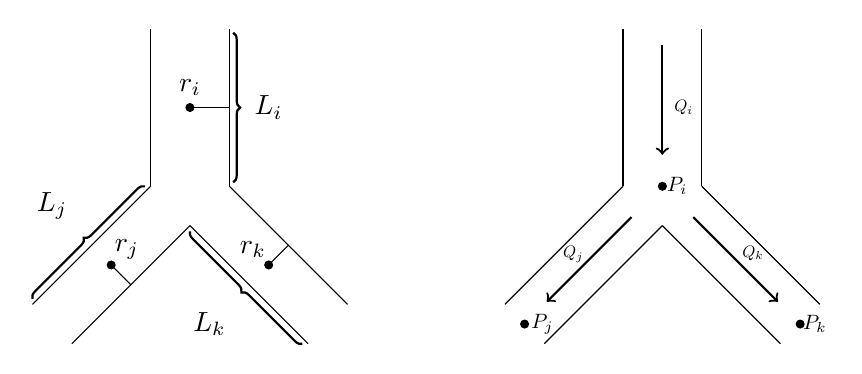
\begin{tikzpicture}
            
% airway drawn as:
%
%    #1 ----------- #2
%          (air)
%    #3 ----------- #4
\def\drawairway(#1)(#2)(#3)(#4){
    \draw[thin] (#1) -- (#2);
    \draw[thin] (#3) -- (#4);
}
\def\drawradius(#1)(#2)[#3]#4{
    \filldraw (#1) circle (.05);
    \draw[thin] (#1) -- (#2) node[pos=0,#3] {#4};
}
\def\drawlength(#1)(#2)[#3]#4{
    \draw[thick,decorate,decoration={brace,raise=.5mm,pre=moveto,pre length=.5mm,post=moveto,post length=.5mm}]
        (#1) -- (#2) node[pos=0.5,#3] {#4};
}

%           [#3]{#4}
%    #1  ------------->  #2 o [#5]{ #6 }
\def\drawflowandpressure(#1)(#2)[#3]#4[#5]#6{
    \draw[->,thick,shorten <=2mm,shorten >=4mm] (#1) -- (#2) node[pos=.5,scale=.6,#3] {#4};
    \filldraw (#2) circle (.05);
    \node at (#2) [scale=.75,#5] {#6};
}

%%% Left-hand info

% parent airway
\drawairway(1.5,2)(1.5,4)(2.5,2)(2.5,4)
\drawradius(2,3)(2.5,3)[yshift=.25cm]{$r_i$}
\drawlength(2.5,4)(2.5,2)[xshift=.5cm]{$L_i$}
% left branch
\drawairway(0,.5)(1.5,2)(.5,0)(2,1.5)
\drawradius(1,1)(1.25,.75)[yshift=.2cm,xshift=.2cm]{$r_j$}
\drawlength(0,.5)(1.5,2)[xshift=-.5cm,yshift=.5cm]{$L_j$}
% left branch
\drawairway(3.5,0)(2,1.5)(4,.5)(2.5,2)
\drawradius(3,1)(3.25,1.25)[yshift=.2cm,xshift=-.2cm]{$r_k$}
\drawlength(3.5,0)(2,1.5)[xshift=-.5cm,yshift=-.5cm]{$L_k$}

%%% Right-hand info (x+6)

% parent airway
\drawairway(7.5,2)(7.5,4)(8.5,2)(8.5,4)
\drawflowandpressure(8,4)(8,2)[xshift=4.5mm]{$Q_i$}[xshift=2.5mm]{$P_i$}
% left branch
\drawairway(6,.5)(7.5,2)(6.5,0)(8,1.5)
\drawflowandpressure(7.75,1.75)(6.25,.25)[xshift=-2.2mm,yshift=2.2mm]{$Q_j$}[xshift=3mm]{$P_j$}
% right branch
\drawairway(9.5,0)(8,1.5)(10,.5)(8.5,2)
\drawflowandpressure(8.25,1.75)(9.75,0.25)[xshift=2.5mm,yshift=2.5mm]{$Q_k$}[xshift=2.5mm]{$P_k$}

        \end{tikzpicture}
        \subcaption{
            Bifurcation from parent branch $i$ to children $j$ and $k$, both dimensions (left) and
            state (right).
    }
    \end{subfigure}
    \par\bigskip
    \begin{subfigure}[t]{.4\textwidth}
        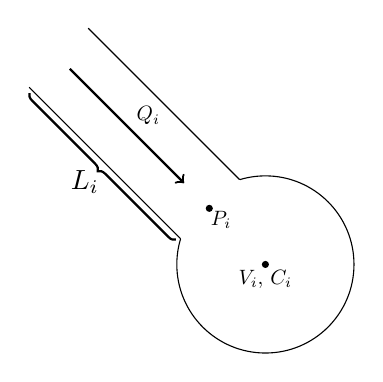
\begin{tikzpicture}[scale=.75]
            % A path that follows the edges of the current page
%    https://tex.stackexchange.com/a/12033
\tikzstyle{reverseclip}=[insert path={(current page.north east) --
  (current page.south east) --
  (current page.south west) --
  (current page.north west) --
  (current page.north east)}
]

\begin{scope}
    \begin{pgfinterruptboundingbox}
        \path[clip] (0,4.5) -- (3.5,1) -- (4.5,2) -- (1,5.5) [reverseclip];
    \end{pgfinterruptboundingbox}
    \draw (4,1.5) circle (1.5);
\end{scope}

\begin{scope}
    \begin{pgfinterruptboundingbox}
        \path[clip] (4,1.5) circle (1.5) [reverseclip];
    \end{pgfinterruptboundingbox}
    \draw (0,4.5) -- (3.5,1) -- (4.5,2) -- (1,5.5);
\end{scope}

\filldraw (4,1.5) circle (.05);
\node at (4,1.5) [scale=.75,yshift=-.25cm] {$V_i,\,C_i$};
\draw[->,thick,shorten <=2mm,shorten >=4mm] (.5,5) -- (3,2.5) node[pos=.5,xshift=.2cm,yshift=.2cm,scale=.75] {$Q_i$};
\filldraw (3.05,2.45) circle (.05);
\node at (3,2.5) [scale=.75,yshift=-.25cm,xshift=.25cm] {$P_i$};
\draw[thick,decorate,decoration={brace,raise=.5mm,pre=moveto,pre length=.2mm,post=moveto,post length=.5mm}]
    (2.55,1.95) -- (0,4.5) node[pos=.5,xshift=-.25cm,yshift=-.25cm] {$L_i$};

        \end{tikzpicture}
        \subcaption{Acinar region and attached branch}
    \end{subfigure}
    \caption{
        2-dimensional cross-section of a modelled bifurcation (a) and acinar region (b), labelled
        with the values composing the equations in \autoref{sec:simultaneous-equations}.
    }
\end{figure}

\subsection{Modelling in the abstract} \label{sec:modelling-in-the-abstract}

We use an \textit{implicit} Euler method to model the system as it progresses: at each timestep, our
simulation updates its state to the value of an approximate solution to the system of equations
above. \autoref{eq:volume-cons-naive} provides the necessary bounds to make the method implicit,
giving us higher accuracy at the cost of implementation complexity.

To solve for an approximate solution at each timestep, we use Newton's method with $f_{\bm{S}}(\bm{x})$ as
defined below, iterating until $\norm{f_{\bm{S}}(\bm{x})}^2 \le tol$ and $\norm{dx}^2 \le tol$, with
a tolerance of $10^{-6}$. The two ``inputs''~--~$\bm{S}$ and $\bm{x}$~--~partition the state of the
model into the variables that are controlled externally (e.g.: pleural pressure, compliance) and
those that are calculated from the system state (e.g.: acinar volume, airflow). The definitions of
$\bm{x}$ and $f_{\bm{S}}$ are given by:

\begin{equation*}
    x = (P_i..., Q_i..., V_i...)
\end{equation*}

\begin{equation*}
    f_{\bm{S}}(\bm{x}) =
        \begin{bmatrix}
            P_{\text{parent}(i)} - P_i - R(i)Q_i \\
            \vdots \\
            Q_i - \sum Q_{\text{child}} \\
            \vdots \\
            V_i^t - V_i^{t-1} - dtQ_i^t \\
            \vdots \\
            P_i - P_{pl}(t) - \frac{1}{C_i} V_i \\
            \vdots \\
        \end{bmatrix}
\end{equation*}

Note that the values in $\bm{x}$ and equations in $f$ are repeated only as many times as fits; e.g.,
there are fewer acinar regions than total branches, so there are fewer components in $\bm{x}$ from
each $V_i$ than from each $Q_i$.

As $\bm{S}$ only exists in the abstract sense, we won't bother to define its structure; all that's
necessary to know is that it contains every variable referred to in $f$ that is not already given
explicitly by $\bm{x}$.

\breakpars

It's worth noting that in practice, the above definitions are only \textit{nearly} correct; a few
adjustments were made to the inputs and equations to mitigate limitations from floating-point
accuracy. These are discussed in the \hyperref[sec:modified-equations]{next section}.

\subsection{Modified equations for floating-point accuracy} \label{sec:modified-equations}

During initial experimentation, it became apparent that~--~under certain conditions~--~the pressure
differential between ends of the bronchial tubes became too small for floating-point calculations to
represent the changes in pressure during updates from Newton's method. This was because the absolute
magnitude of the pressure (around 1e6 Pascals) was significantly different from the differences in
pressure (much less than 1 Pascal).\footnotemark\ We mitigated this by changing the formulation of
the equations used in the simulation, improving their accuracy without changing their semantic
meaning.

\footnotetext{
    \textbf{N.B.:} The change in pressure from \textit{timestep-to-timestep} was still large enough
    to represent, but the changes to $dx$ during the Newton iteration were. While it initially
    resolved by the methods in this section, this problem would have also been far lesser with
    64-bit floating-point values (which we did eventually switch to).

    \noindent
    Please also note: The approximate pressures described here might be, but are not necessarily,
    reflective of pressures in the final simulation; there were multiple issues fixed after this
    observation that may have impacted these values. Even still, the modification was kept, as it
    provided a non-zero benefit.

    \noindent
    This problem was detected while simulating unrestricted models, where the relative ease of flow
    means that the pressure throughout the lungs remains much more balanced.
}

The ``new'' equations gain accuracy by centering values closer to a magnitude of 1, so that the
required number of significant digits is greatly reduced.\footnotemark\ These equations use two new
values, $\hat{P}$ and $\hat{V}$, that are relative to atmospheric pressure. They are defined by:

\footnotetext{
    Floating-point numbers have a fixed number of significant digits; arithmetic operations with
    large differences in magnitude tend to lose significant information in the process.
}

\begin{equation}
    \hat{P} = P - P_{\text{atm}}
\end{equation}

\noindent
where $P_{\text{atm}}$ is is atmospheric pressure; and:

\begin{align}
    \hat{V} & = V - V \vert_{P = P_{\text{atm}}} \\
            & = C (\hat{P} - P_{pl})
\end{align}

\noindent
Note that the definition of $\hat{V}$ would be the result of simply substituting $\hat{P}$ for $P$
in \autoref{eq:volume-cons-naive}. Applying these substitutions gives the following equations,
equivalent to their counterparts above:

\begin{equation}
    \hat{P}_{\text{parent}} - \hat{P}_i = R(i) Q_i
\end{equation}

\begin{equation}
    Q_i = \sum Q_{\text{child}}
\end{equation}

\begin{equation}
    \hat{V}_i^t = \hat{V}_i^{t-1} + dt Q_i^t
\end{equation}

\begin{equation}
    \hat{P}_i = \frac{1}{C_i} \hat{V}_i + P_{pl}(t)
\end{equation}

Representing the pressure and volume by their \textit{offset} from values at atmospheric pressure
causes them to cluster much closer to zero~--~the magnitude of the mean is significantly decreased,
relative to the variance of the values. This of course greatly improves the accuracy of each Euler
step.

The same substitutions also apply to our representations of the state of the model and the
optimization function used for Newton's method, as shown in \autoref{sec:modelling-in-the-abstract}.

\subsection{Sparse matrices} \label{sec:sparse-matrices}

A key observation that aiding in simulation speed is that the Jacobian of our optimization function
$f$ has only $\mathcal{O}(n)$ entries~--~which allows for dramatic storage space and runtime
savings. This optimization is crucial for practically running simulations up to a high depth on a
single computer.

We used sparse matrices, solving the equations with a sparse Gaussian elimination. Other methods
(such as GMRES) were initially considered but not used, due in equal parts to lack of library
support and the sufficiency of the simpler Gaussian elimination.\footnotemark\ The increase in
execution speed from dense to sparse matrices is quite significant, as demonstrated in
\autoref{fig:sparse-speed}. The observed time for a simulation tick~--~which is roughly proportional
to the time spent solving the system of equations~--~is still not linear in the number of nodes,
however: fitting the sparse matrix timings to a power series model gives an exponent of 1.97 and
$R^2$ of 0.989. Fitting a power series to the dense matrix timings gives an exponent of 3.35 and
$R^2$ of 0.997; clearly significantly worse.

\footnotetext{
    There are, of course, \textit{many} sparse matrix libraries in existence. The project was
    written in Rust, which~--~at time of writing~--~did not have more advanced sparse matrix
    solvers.
}

\begin{figure}[p!]
    \centering
    \begin{tikzpicture}
        \input{figs/sparse-speed-comparison.tex}
    \end{tikzpicture}
    \caption{
        Time to compute a single simulation tick, with dense versus sparse matrices. Models were
        simulated for 10 ticks in total, with the results above taken as the average of the final 5,
        to reduce the impact of operating system caching on performance.
    }
    \label{fig:sparse-speed}
\end{figure}

% todo: fix formatting of text in subcaptions here.
\begin{figure}[p!]
    \centering
    \begin{subfigure}[t]{.47\textwidth}
        \centering
        \tightbox{\includegraphics[width=.9\linewidth]{figs/sparse/separate-rev-big.png}}
        \caption{ The sparsity pattern of Jacobians as implemented }
        \label{subfig:sparse-organization-implemented}
    \end{subfigure}%
    \hspace{1em}%
    \begin{subfigure}[t]{.47\textwidth}
        \centering
        \tightbox{\includegraphics[width=.9\linewidth]{figs/sparse/branchgroup-big.png}}
        \caption{
            A possible ``cleaner'' sparsity pattern, arranging variables for each node at
            consecutive indexes.
        }
        \label{subfig:sparse-organization-hypothetical}
    \end{subfigure}
    \caption{
        Comparison of the implemented sparsity pattern with one possible alternative (of many).
        \ref{subfig:sparse-organization-hypothetical} is not \textit{necessarily} more efficient; it
        demonstrates that other options were available, as an area of possible improvement.
    }
    \label{fig:sparse-organization}
\end{figure}

Although the improvement from $\mathcal{O}(x^{3.35})$ to $\mathcal{O}(x^{1.97})$ is significant, it
is possible that other orderings of values within the Jacobian may be better-optimized for sparse
Gaussian elimination. \autoref{fig:sparse-organization} provides a visual comparison between the
sparsity pattern that was used in the software developed for this paper and a hypothetical
alternative. The current layout used places all variables and equations of a certain type at
consecuitve indexes, i.e. $(P\dots, Q\dots, V\dots)$ instead of e.g.
$(P_0,Q_0,V_0,\,P_1,Q_1,V_1,\,\dots)$, with variables and equations for parent nodes occuring at
\textit{later} indexes.

As context for \autoref{fig:sparse-organization} however, it is important to note that it is not
possible for the system of equations to be simply organized into an upper- or lower-triangular
matrix; each equation is composed of at least two variables. With this option unavailable, we did
not assess alternate orderings of values within the Jacobian.

\subsection{Procedural lung generation \& configuration} \label{sec:procedural-generation}

As part of the simluation software developed for this paper, there are a number of configurable
parameters~--~primarily encapsulating the structure of the lungs and how they change over the course
of the simulation. Listing them exhaustively, the parameters are:

\begin{itemize}
\item Lung structure (the tree formed by the relationship between branches)
\item Approximate typical lung FRC
\item Branch length, as relative to the parent
\item Branch radius (healthy \& degraded), relative to the parent
\item Acinar region \textit{relative compliance} (healthy \& degraded)
\item Branch angles (only affects the lungs' appearance)
\item Keyframe-based scheduling to shift the lung state between healthy \& degraded
    \begin{itemize}
    \item Multiple interpolation functions to transition between keyframes
    \end{itemize}
\item Pleural pressure wave characteristics (initial value, mean, amplitude, and period), as well as
    the ``normal'' maximum value (see below).
\end{itemize}

The specification of ``healthy'' and ``degraded'' allows us to define and transition between two
states of the lungs, simulating the onset and treatment of the affects from many respiratory
illnesses. The speed of onset or recovery is controlled by the positioning of the keyframes, which
are binary ``healthy'' or ``degraded'' states. These states do not directly affect the simulation
state, i.e. the flow, pressure, and acinar volume within each branch. This does mean that, for
example, the pressure in constricting airways does not increase directly as a result of that
constriction, but we have considered the volume inside the branches themselves largely negligible.
The most important factor is that the volume within each acinar region is conserved, which
\textit{is} guaranteed, even across changing compliance.

\breakpars

It is also worth clarifying the meaning of \textit{relative compliance} in the list above. In order
to ensure that the total volume of the lungs remains consistent with human anatomy, the compliance
of each acinar region is linearly scaled so that the total volume from all acinar regions filled at
atmospheric pressure would give the configured FRC of the lungs at the ``normal'' maximum pleural
pressure (a separately-configurable value). For typical values (e.g. those described in
\autoref{sec:results}), the total lung compliance is approximately $2.0 \times 10^{-6}
\text{m}^3/\text{Pa}$ (approximately 0.2 L/cm\ce{H_2O}).

\breakpars

The details of the configuration format itself are outside the scope of this paper, but the
configurable values are described here to provide context for the parameters that were varied in the
experiments we report. A number of these parameters actually were never experimented with, due to
scope of the project.

\subsection{Interpolation functions} \label{sec:interpolation}

\begin{figure}[ht!]
    \centering
    \begin{tikzpicture}
        \begin{axis}[
    align=center,
    title={Selected interpolation functions},
    xmin=0, xmax=1,
    ymin=0, ymax=1,
    domain=0:1,
    xtick={0,0.2,0.4,0.6,0.8,1},
    ytick={0,0.2,0.4,0.6,0.8,1},
    legend pos=south east,
    width=.6\textwidth,
    every axis plot/.append style={thick},
]

    \addplot[mark=none,color=softred,samples=2] { x };
    \addlegendentry{Linear}

    \addplot[mark=none,color=softgreen,samples=300] { .5 * tanh(6*x-3)/tanh(3) + .5 };
    \addlegendentry{Tanh}
    
    \addplot[mark=none,color=softblue,samples=300] { .5 * (1 - cos(pi * deg(x))) };
    \addlegendentry{Trigonometric}
    
    \addplot[mark=none,color=softorange,samples=300] { 3*x^2 - 2*x^3 };
    \addlegendentry{Cubic}

\end{axis}

    \end{tikzpicture}
    \caption{Comparison of the four selected interpolation functions}
    \label{fig:interpolate-functions}
\end{figure}

A number of later experiments transition between differing levels of airway constriction with the
use of \textit{keyframes}~--~a set of $(\text{time}, \text{constriction})$ pairs defining a handful
of states that must be reached. To define the intermediate values between these states, we have four
different interpolation functions:

\begin{itemize}
    \item \textit{Linear}: $f(x) = x$
    \item \textit{Tanh}: $f(x) = \frac{1}{2} \frac{\tanh(6x - 3)}{\tanh(3)} + \frac{1}{2}$
    \item \textit{Trigonometric}: $f(x) = \frac{1}{2} (1 - \cos(\pi x))$
    \item \textit{Cubic}: $f(x) = 3x^2 - 2x^3$
\end{itemize}

\noindent
A visual comparison of these functions is provided in \autoref{fig:interpolate-functions}.

These functions were selected as options for their relative simplicity and variety of curvatures.
While we could change these parameters instantaneously, there were a couple reasons to have smooth
transitions~--~primarily to avoid instantaneous jumps in flow or volume, but also because processes
that would affect the lungs in this way are very unlikely to be instantaneous themselves. If we
\textit{do} need to model a near-instant change, keyframes already allow us to make the transition
period arbitrarily short.

Some amount of curvature is also desirable~--~although perhaps not necessary: without a continuous
derivative, there are often unusually sharp changes in the rate of flow. This is perhaps intuitive,
but still worthwhile to point out.

Finally, it is worth noting that the correction factor of $\tanh(3)$ in the denominator of the
\textit{Tanh} interpolation function is nearly equal to 1, but still necessary. The value of
$\tanh(3)$ is only 0.995, but experiments without that correction factor showed clearly visible
jumps in the rate of flow from that small change. While these changes were most likely harmless, we
still elected to remove them.
